\documentclass[
  final,
  babelLanguage=portuguese,
  %desktopVersion,
  %showtrims,
  %overleaf,
]{anecdote}

%\graphicspath{{./assets/photos/300dpi/}}
%\graphicspath{{./assets/photos/92dpi/}}

% NOTE: pdfinfo tags and hyperref metadata are set in the documentclass.

% Page size: 6x9 inch
% Body text: 10.5 / 15 pt

\usepackage{local}

%% Details of the book
%% ===================

\title{Meditação a Andar}
\subtitle{}
\author{Ajahn Nyanadhammo}
\publisher{Publicações Sumedhārāma}
\date{2017-08-20}
\editionInfo{\emph{Segunda Edição}, impresso na Malásia, 2018}
\ISBN{978-989-8691-65-1}

% === Metadata ===

\pdfinfo{%
  /Title (\thetitle)%
  /Author (\theauthor)
  /Subject (Meditação a Andar)
  /Keywords (buddhism, Dhamma, meditação)
  /GTS_PDFXVersion (PDF/X-1:2001)%
  /GTS_PDFXConformance (PDF/X-1a:2001)%
}

%% === Load further packages ===

%% === Hyphenation exceptions and corrections ===

\hyphenation{London}

\begin{document}

\frontmatter

\ifdesktopversion
\desktopCover{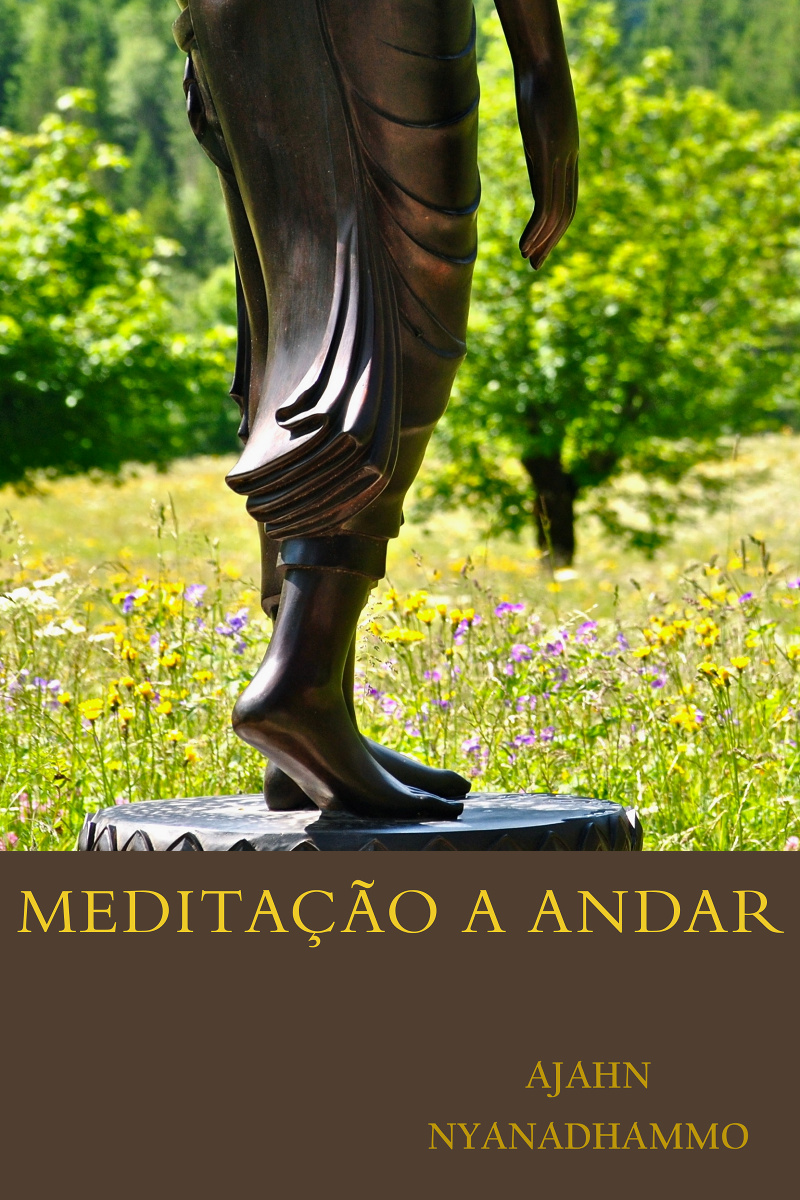
\includegraphics[height=\paperheight]{./desktop-cover.jpg}}
\fi

\cleartorecto
\thispagestyle{empty}
\vspace*{5em}

{\centering

\settowidth{\titleLength}{%
  {\Large\chapterTitleFont\scshape\MakeLowercase{\thetitle}}%
}

{\Large\chapterTitleFont\scshape\MakeLowercase{\thetitle}}\\[0.3\baselineskip]
\setlength{\xheight}{\heightof{X}}
\raisebox{0.5\xheight}{\color[gray]{0.4}\rule{\titleLength}{0.25pt}}\\[0.3\baselineskip]
{\itshape
\thesubtitle}

\vfill

\theauthor

\vspace*{5em}

}



\cleartoverso
\thispagestyle{empty}

{\copyrightsize
\centering
\setlength{\parindent}{0pt}%
\setlength{\parskip}{0.8\baselineskip}%

\thetitle\\
por \theauthor

Publicações Sumedhārāma\\
\href{http://sumedharama.pt}{www.sumedharama.pt}

As publicações de Sumedharama são para distribuição gratuita. Na maioria
dos casos, isto é possível graças a doações, de indivíduos ou grupos,
feitas especificamente para que as publicações dos ensinamentos do
Buddha possam estar disponíveis gratuitamente.

\textit{Sabbadānaṃ dhammadānaṃ jinati}\\
`A oferta de Dhamma é superior a qualquer outra oferta.'

Este livro encontra-se disponível para distribuição gratuita em\\
\href{http://fsbooks.org/}{www.fsbooks.org}

ISBN \theISBN

Copyright \copyright\ Publicações Sumedhārāma 2018

Traduzido por José Megre

Traduzido do original `Walking Meditation -- In the Thai Forest Tradition'

Coppyright \copyright\ The Sangha, Wat Pah Nanachat, 2003

Fotografia da Capa: Ajahn Kancano

Editado a partir de duas palestras de Dhamma oferecidas por
Ajahn Nyanadhammo, no Buddhist Centre Dhammaloka, em 31 de Julho de
1992, e no Bodhinyana Forest Monastery, em 22 de Janeiro de 2002, ambos
em Perth, na Austrália.

\vfill

{\footnotesize

Este trabalho está licenciado com uma Licença Creative Commons\\
Atribuição-NãoComercial-SemDerivações 4.0 Internacional.

Veja página \pageref{copyright-details} para mais detalhes sobre direitos e restrições desta licença.

Produzido com o sistema tipográfico \LaTeX.\\
Fonte utilizada: Gentium e Alegreya.

\theEditionInfo

}}


\cleartorecto
\thispagestyle{empty}

% TODO review dedication

\mbox{}\vfill

\begin{verse}

{\upshape Dedicação}\\[0.4\baselineskip]
Gostaríamos da agradecer a todos aqueles que ajudaram\\
na preparação deste livro, em especial ao grupo Kataññutā\\
da Malásia, de Singapura e da Austrália, impressas\\
para distribuição gratuita.

\end{verse}

\vfill\mbox{}



%% No TOC, the content is very short.
%\cleartorecto
%\tableofcontents*

% Page 1 is the first page of the first chapter.
\mainmatter

\chapter{Introdução}

Nesta palestra, vou concentrar"-me nos aspectos essenciais da meditação a
andar abordando as questões `Como?', `Quando?', `Onde?' e `Porquê?'.
Pretendo incluir instruções práticas sobre os aspectos técnicos da
meditação a andar e instruções para cultivar qualidades mentais que
levam à concentração, introspecção e sabedoria através da actividade
física da meditação a andar.

O Buddha enfatizou o cultivo de um estado consciente nas quatro
principais posturas: de pé, sentado, deitado e a andar (DN 22, MN 10). Ele
encorajou"-nos a desenvolvermos a atenção em todas estas posturas, de forma a termos
consciência e reconhecimento daquilo que estamos a fazer em
qualquer posição.

Se lerem acerca da vida dos monges e monjas no tempo de Buddha,
perceberão que muitos alcançaram certos estágios de iluminação enquanto
praticavam meditação a andar. Meditação a andar chama"-se \emph{caṅkama}
em Pali. É uma actividade que permite focar e concentrar a mente
ou desenvolver conhecimento e sabedoria introspetiva.

Algumas pessoas sentem"-se naturalmente mais atraídas pela meditação a
andar, por a considerarem mais fácil e natural do que a meditação
sentada. Quando se sentam, sentem"-se aborrecidas, tensas ou distraem"-se
facilmente. As suas mentes não se acalmam. Se este é o vosso caso, não
persistam; façam alguma coisa nova e experimentem mudar de postura.

Façam alguma coisa diferente, experimentem a meditação em pé ou tentem a
meditação a andar. Esta nova postura de meditação poderá tornar"-se numa
forma arguta de focar a mente. Todas as quatro posturas de meditação são
apenas técnicas, métodos para desenvolver e treinar a mente.

Experimentem desenvolver a meditação a andar e talvez possam começar a
aperceber"-se dos seus benefícios. Na Tradição da Floresta, no nordeste
da Tailândia, há uma grande ênfase na meditação a andar. Muitos dos
monges desta tradição praticam"-na durante longos períodos, como uma
forma de desenvolver concentração. Por vezes chegam a praticar até dez
ou quinze horas por dia!

O falecido monge Ajahn Singtong praticava tanto a meditação a
andar que chegava a criar um sulco no caminho de meditação. Ele chegava
a caminhar até quinze horas por dia, tornando o arenoso caminho que
usava, côncavo! Outro Monge, Ajahn Kum Dtum, praticava meditação
a andar tão assiduamente que à noite nem se preocupava em entrar na sua
cabana. Quando se sentia realmente cansado de caminhar durante todo o
dia e toda a noite, dormia mesmo ali, no chão, utilizando as mãos como
almofada. Adormecia conscientemente tendo determinado levantar"-se
assim que acordasse. Assim que acordava, continuava a andar novamente.
Basicamente vivia no carreiro de meditação. Ajahn Kum Dtum
alcançou rapidamente resultados na sua prática.

No Ocidente não se costuma falar tanto da meditação a andar, por isso eu
gostaria de descrever o processo e recomendá"-la como complemento à
meditação sentada. Espero que estas instruções vos ajudem a desenvolver
o vosso repertório de técnicas de meditação -- tanto em meditação formal
como na vida quotidiana. Como grande parte da vida é passada a andar, se
souberem como estar conscientes disso, o simples facto de andarem em
casa pode tornar"-se num exercício de meditação.

\section{Os Cinco Benefícios da Meditação a Andar}

O Buddha falou sobre cinco benefícios da meditação a andar (AN. III. 29). Neste
\emph{Sutta}, ordenou"-os da seguinte forma: desenvolve a resistência para
caminhar longas distâncias, desenvolve vigor, previne doenças, ajuda a digestão
após a refeição e a concentração adquirida na meditação a andar é duradoura.

\begin{siderule-quote}
  1. Desenvolve resistência para caminhar longas distâncias
\end{siderule-quote}

O primeiro benefício da meditação a andar consiste no desenvolvimento de
resistência para caminhar longas distâncias. Isto era particularmente
importante na época de Buddha, visto a maioria das pessoas
deslocar"-se a pé. O próprio Buddha deslocava"-se regularmente a
pé, de local para local, chegando a caminhar até dezasseis quilómetros
por dia. Desta forma, ele recomendava a meditação a andar como forma de
desenvolver uma condição física saudável e resistência para percorrer
longas distâncias.

Ainda hoje, os monges da floresta fazem longas caminhadas, às quais se
chama \emph{Thudong} (\emph{dhutanga}). Agarram nas suas tigelas de
oferendas e nos seus mantos e partem à procura de lugares isolados para
meditar. Como preparação antes de partirem, aumentam progressivamente as
horas de prática da meditação a andar até um mínimo de cinco ou seis
horas por dia, com o intuito de desenvolverem aptidão física e
resiliência. Se andarem cerca de quatro a cinco quilómetros por hora e
praticarem cinco horas de meditação a andar por dia, o número de
quilómetros vai"-se acumulando.

\begin{siderule-quote}
  2. Desenvolve vigor
\end{siderule-quote}

O desenvolvimento de vigor, especialmente para superar sonolência, é o
segundo benefício da meditação a andar. Enquanto praticam meditação
sentada, as pessoas notam que existe tendência para entrar em estados
tranquilos, mas se estiverem demasiado tranquilos, sem estarem conscientes,
podem começar a adormecer, chegando mesmo a ressonar! O tempo passa
rapidamente, e apesar de ser apaziguador, não existe claridade ou
consciência. Sem atenção nem consciência, a meditação pode
tornar"-se aborrecida pois é dominada por preguiça e sonolência.
Desenvolver a meditação a andar pode contrariar esta tendência.

Como exemplo, Ajahn Chah recomendava que, uma vez por semana,
ficássemos acordados toda a noite, meditando e caminhando. Normalmente
ficamos bastante sonolentos à uma ou duas da madrugada, por isso,
Ajahn Chah recomendava fazermos meditação a andar de costas, para
contrariar o sono. Não se adormece a andar de costas!

Quando estava no Mosteiro \emph{Bodhinyana}, no oeste da Austrália,
lembro"-me de sair uma manhã cedo, por volta das cinco horas, para
praticar meditação a andar. Vi um dos leigos que tinha passado o Retiro
das Chuvas (vassa) no mosteiro, a fazer um esforço enorme para superar a
sonolência. Ele estava a praticar meditação a andar em cima de um muro
com dois metros de altura, que existia em frente ao mosteiro -- andava
muito conscientemente para trás e para a frente em cima do muro! Eu estava
um pouco preocupado que ele pudesse cair e magoar"-se. Contudo, ele
estava a fazer um grande esforço para estar atento a cada passo,
desenvolvendo um elevado estado de alerta, esforço e empenho para
superar a sonolência.

\begin{siderule-quote}
  3. Previne doenças
\end{siderule-quote}

O Buddha disse que a meditação a andar mantém"-nos saudáveis. É o
terceiro benefício. Todos temos consciência que andar é considerado uma
óptima forma de exercício físico. Hoje em dia até ouvimos falar sobre
``\emph{power walking}'' (forma de exercício físico em que se caminha de
maneira rápida e vigorosa). Aqui, estamos a falar de ``\emph{power
meditation}'', ou seja, desenvolver a meditação a andar como exercício
físico e também mental. Desta forma, caminhar não é só uma boa forma de
exercício físico, mas também nos ajuda a cultivar a mente. No entanto,
para usufruirmos destes dois benefícios, temos que estar conscientes do processo de caminhar, em vez de deixarmos a mente dispersar"-se ao pensar
noutras coisas.

\begin{siderule-quote}
  4. Facilita a digestão após a refeição
\end{siderule-quote}

O quarto benefício da meditação a andar é ajudar a digestão. Para os
monges, que apenas têm uma refeição por dia, este facto é
particularmente importante. Depois de uma refeição, o sangue flui para o
estômago, distanciando"-se do cérebro, o que pode provocar sonolência. Os
Monges da Floresta salientam que, após uma refeição, deve"-se praticar
algumas horas de meditação a andar para facilitar a digestão. Para os
praticantes leigos aplica"-se o mesmo. Depois de uma refeição pesada, em
vez de fazer"-se uma sesta, deve"-se sair e praticar uma hora de meditação
a andar. Ajuda o bem"-estar físico e é uma boa oportunidade de exercitar
a mente.

\begin{siderule-quote}
  5. A concentração adquirida na meditação a andar é duradoura
\end{siderule-quote}

O quinto benefício da meditação a andar é que a concentração gerada por
esta prática mantém"-se por muito tempo. A postura em andamento é na
realidade uma postura pouco refinada em comparação com a postura sentada
no que se refere à actividade envolvida. Enquanto sentados, é fácil
mantermos essa posição; temos os olhos fechados, por isso não estamos
sujeitos a estímulos visuais e não estamos ocupados com o movimento do
corpo. O mesmo é verdade para as posturas de pé e deitado pois estas
também não implicam movimento.

Enquanto caminhamos há muita estimulação sensorial devido ao movimento
do corpo e de estarmos a ver para onde nos dirigimos (estimulação
visual). Portanto, se conseguirmos concentrar a mente enquanto andamos e
recebemos todos estes estímulos sensoriais, então, quando mudamos desta
postura para uma mais refinada, será mais fácil manter a concentração.
Isto é, quando nos sentamos, a energia mental e o poder de concentração
irão facilmente ser transferidos para esta postura mais refinada.

Pelo contrário, se apenas desenvolvemos a concentração na postura
sentada, quando nos levantamos e iniciarmos movimentos corporais mais
evidentes, como o andar, é difícil mantermos o estado de concentração.
Isto acontece porque estamos a transitar de posturas mais refinadas para
menos refinadas. Assim, a meditação a andar pode ajudar a desenvolver
energia, clareza mental e uma concentração que continua noutras
posturas, menos activas, de meditação.



\chapter{Preparação Para a Prática da Meditação a Andar}

\section{Encontrar um local adequado}

O local, onde o Senhor \emph{Buddha} praticava a meditação a andar depois de
atingir a Iluminação, em \emph{Bodhgaya}, ainda existe nos dias de hoje. O
trajeto onde ele praticava esta forma de meditação tinha dezassete passos de
comprimento. Atualmente, os Monges da Floresta tendem a fazer trajetos mais
compridos. Podem ter até trinta passos. Os principiantes podem achar esta
distância um pouco longa, pois ainda não têm a concentração desenvolvida. Quando
chegam ao fim do trajeto, a mente pode já ter dado a volta ao mundo e
regressado. Lembrem-se que caminhar é estimulante e que inicialmente a mente
tende a dispersar-se. Normalmente, é melhor os principiantes começarem com um
trajeto mais curto: quinze passos seria uma distância ideal.

Se praticarem meditação ao ar livre, tentem fazê-lo num local isolado
onde não se distraiam, nem sejam facilmente perturbados. É aconselhável
encontrarem um local para a praticar que seja ligeiramente abrigado.
Poderá ser uma distração caminhar numa zona aberta com paisagem, pois a
mente poderá ser atraída pelo cenário. Uma zona abrigada é especialmente
adequada para pessoas que têm tendência para pensar muito, ajudando-as a
acalmar a mente (Vsm, III, 103). Se praticarem num local fechado, a
mente tende a voltar-se para dentro, para o próprio ser, ao encontro da
paz.

\section{Preparar o corpo e a mente}

Quando tiverem escolhido o trajeto adequado, coloquem-se num dos
extremos do trajeto. Mantenham-se direitos. Coloquem à frente do vosso
corpo a mão esquerda e por cima dela a mão direita. Não andem com as
mãos atrás das costas. Lembro-me de um mestre de meditação, que quando
visitou o mosteiro e ao ver um dos visitantes a andar para trás e para a
frente com as mãos atrás das costas, fez o seguinte comentário: ``Ele
não está a praticar meditação a andar, está a passear''. O mestre fez
esta observação porque reparou que não havia uma determinação clara de
focar a mente na meditação a andar, na qual se coloca as mãos à frente
do corpo para distinguir o que estamos a fazer de um simples passeio.

O objetivo primário da prática é desenvolver \emph{samādhi}, e isto
requer esforço focalizado. A palavra em \emph{Pāḷi,} \emph{samādhi,}
significa focar a mente, ou desenvolver a mente até esta se encontrar
unificada através de níveis graduais de atenção e concentração. Para
focarmos a mente necessitamos ser diligentes e determinados. Em primeiro
lugar, é necessário um certo grau de compostura física e mental.
Começamos esta compostura unindo as mãos à nossa frente, tranquilamente.
Uma postura calma do corpo ajuda a compor a mente. Assim, com o corpo
tranquilo, devem permanecer quietos e trazer a consciência e a atenção
para o corpo. Depois, levantem as mãos conjuntamente em \emph{añjali},
um gesto de respeito no qual une-se verticalmente as palmas das mãos em
frente do peito, e com os olhos fechados reflitam durante alguns minutos
nas qualidades do \emph{Buddha}, do \emph{Dhamma} e do \emph{Sangha}
(\emph{Buddhanussati}, \emph{Dhammanussati} e \emph{Sanghanussati}).

Podem contemplar o facto de terem tomado refúgio no \emph{Buddha},
aquele que é Sábio, aquele que Vê e Conhece, o Desperto, o Iluminado.
Reflitam por alguns minutos, com o vosso coração, nas qualidades do
\emph{Buddha}. Depois recordem-se do \emph{Dhamma} -- a Verdade que
estão a tentar realizar e desenvolver ao praticarem meditação a andar.
Finalmente, tragam à mente o \emph{Sangha} -- especialmente os
Despertos, que realizaram a verdade praticando meditação. Depois ponham
as mãos em baixo à vossa frente e determinem mentalmente durante quanto
tempo irão praticar meditação a andar, seja meia hora, uma hora ou mais.
Independentemente do tempo que determinaram para a prática,
mantenham-no. Deste modo, nesta fase inicial da meditação, estão a
alimentar a mente com entusiasmo, inspiração e confiança.

É importante lembrarem-se de olhar para o chão, cerca de um metro e meio
à vossa frente. Mantenham o olhar fixo, não se deixem distrair, seja o
que for que aconteça à vossa volta. Estejam conscientes do que sentem na
planta dos pés, e desenvolvendo assim uma atenção mais refinada e
sabendo claramente que estão a andar, enquanto andam.



% Was: Objetos De Meditação Para Meditação a Andar

\chapter{Objectos}

O Buddha mencionou quarenta objectos de meditação diferentes nos
seus ensinamentos (Vsm, III, 104), muitos dos quais podem ser utilizados
na meditação a andar. Contudo, uns são mais adequados que outros. Irei
examinar aqui alguns desses objectos de meditação, começando por aqueles
utilizados com mais frequência.

\begin{siderule-quote}
  Consciência da postura
\end{siderule-quote}

Neste método, enquanto caminhamos dirigimos toda a atenção para a planta
dos pés, reparando nas sensações conforme elas surgem e cessam (isto é,
presumindo que caminham descalços como faz a maioria dos monges, embora
se necessário possam usar sapatos com sola fina). Assim que começam a
andar, a sensação muda. Quando levantam e pousam o pé, pondo"-o em
contacto novamente com o solo, surge uma nova sensação. Estejam
conscientes desta sensação assim que ela surge na planta do pé. Quando o
pé se levanta de novo, tomem mentalmente nota da nova sensação, assim
que ela surge. Sempre que levantam e pousam cada pé, estejam conscientes
das sensações. A cada novo passo, novas sensações surgem e velhas
sensações cessam. Elas devem ser reconhecidas conscientemente. A cada
passo, novas sensações são experienciadas -- uma sensação surge, uma
sensação cessa; uma sensação surge, uma sensação cessa.

Com este método, mantemos a consciência na sensação de andar, para cada
passo dado, para \emph{vedanā} (sensações agradáveis, desagradáveis ou
neutras). Estamos conscientes de qualquer tipo de \emph{vedanā} que
surge na planta dos pés. Quando estamos de pé, existe uma sensação de
contacto com o solo. Este contacto pode originar dor, calor ou outro
tipo de sensações. Dirigimos a nossa atenção consciente para estas sensações,
reconhecendo"-as. Quando levantamos um pé, a sensação muda assim que
perdemos o contacto com o solo. Quando baixamos o pé, assim que este
entra de novo em contacto com o solo, uma nova sensação surge. Enquanto
andamos, as sensações mudam constantemente, umas cessam e novas surgem.
Conscientemente, reparem no aparecimento e desaparecimento das
sensações na sola dos pés enquanto os levantam e pousam no chão. Assim
toda a atenção é dirigida apenas para as sensações que surgem enquanto
caminhamos.

Alguma vez repararam nas sensações que surgem nos pés enquanto caminham?
Acontecem sempre que andamos, mas normalmente não reparamos nestas
coisas subtis durante a nossa vida. Enquanto caminhamos a mente
normalmente encontra"-se noutro lugar qualquer. A meditação a andar é uma
forma de simplificar o que estamos a fazer enquanto o fazemos. Trazemos
a mente para o ``aqui e agora'', e assim estamos conscientes de estar a
andar, enquanto andamos. Ao reconhecermos apenas as sensações que surgem
e cessam, a mente fica tranquila, tornando tudo mais simples.

A que velocidade se deve caminhar? Ajahn Chah recomendava que
andássemos naturalmente, nem muito depressa, nem muito devagar. Se
caminharem muito depressa, poderá ser difícil concentrarem"-se nas
sensações que surgem e cessam. Podem precisar de caminhar mais
lentamente. Por outro lado, há outras pessoas que podem precisar de
caminhar mais depressa. Depende de indivíduo para indivíduo. Encontrem o
vosso próprio ritmo, aquele que funcionar melhor, seja ele qual for.
Podem começar com um ritmo lento e irem aumentando gradualmente, até
atingirem o ritmo normal de andamento.

Se a vossa concentração é fraca (isto é, se a mente dispersa"-se facilmente),
então andem muito devagar, até conseguirem estar no momento presente a
cada passo dado. Comecem por estabelecer a consciência, no início do
trajecto, e quando chegarem a meio do trajecto perguntem, ``Onde está a minha
mente? Está consciente das sensações na planta dos pés? Estou a notar o
contacto aqui e agora, no momento presente?" Se a mente estiver a
vaguear, então tragam"-na de volta, reparando novamente nas sensações na
planta dos pés, e continuem a caminhar.

Quando chegarem ao fim do trajecto voltem"-se devagar e restabeleçam a atenção novamente. Onde está a mente? Está a aperceber"-se das sensações
na planta dos pés? Ou vagueou? A mente tende a dispersar"-se para outros
lugares, indo atrás de pensamentos de ansiedade, medo, felicidade,
tristeza, preocupações, dúvidas, prazeres, frustrações e muitos outros
que possam surgir. Se não tiverem a atenção plenamente estabelecida no
objeto de meditação, restabeleçam"-na antes de recomeçarem a andar.
Restabeleçam a mente no simples acto de andar e voltem para trás
caminhando até ao fim do trajecto. Quando chegarem a meio deverão
reparar, ``Agora estou a meio caminho'' e confirmem novamente para se
certificarem que a mente está focada no objeto de meditação. Depois,
quando chegarem ao final do trajecto reparem mentalmente, ``Onde está a
mente?" Desta forma, andam para trás e para a frente, plenamente
conscientes das sensações que vão surgindo e cessando. Enquanto
caminham, restabeleçam constantemente a concentração, trazendo a mente de
novo para o interior, retomando o estado consciente, estando conscientes e
reconhecendo as sensações a cada momento, assim que surgem e cessam.

Enquanto estamos conscientes das sensações que sentimos na planta dos
pés, notamos que a mente se distrai menos, que não tem tanta tendência a
distrair"-se com as coisas que estão a acontecer à volta. Ficamos mais
calmos e a mente fica tranquila. Quando a mente fica calma e tranquila,
irão reparar que a postura de meditação a andar se torna numa actividade
demasiado agitada para uma mente com estas qualidades. Vão querer estar
quietos. Então parem e permitam à mente experienciar essa calma e
tranquilidade. Este estado é conhecido como \emph{passaddhi}, que é um
dos factores da Iluminação.

Se enquanto andarem, a mente entrar num estado muito refinado, poderão
sentir que é impossível continuar. Para andar é necessário a vontade de
se moverem, e possivelmente a vossa mente encontra"-se demasiado focada
no objecto de meditação para continuar. Então parem de andar e pratiquem
meditação em pé. Meditação tem a ver com o trabalho da mente e não com
uma postura específica. A postura física utilizada é apenas uma forma de
potencializar o trabalho da mente.

Concentração e tranquilidade funcionam em conjunto com a consciência.
Juntamente com a energia, investigação do Dhamma, alegria e
equanimidade, estes são os ``Sete Fatores da Iluminação."
Quando
meditamos a mente está tranquila, e é devido a esta mesma
tranquilidade que surgem os estados de alegria, êxtase e beatitude. O
Buddha disse que a beatitude da paz é a felicidade suprema (MN, I, 454),
e uma mente concentrada experiencia essa paz. Esta paz pode ser
experienciada nas nossas vidas.

Tendo desenvolvido a prática da meditação a andar num contexto formal,
então quando estivermos a andar na nossa vida diária, a ir às compras, a
ir de um quarto para o outro, ou mesmo a andar até a casa de banho,
podemos praticar meditação a andar. Podemos estar conscientes de estar a
andar, simplesmente tendo isso presente. As nossas mentes podem estar
calmas e em paz. Esta é uma forma de desenvolvermos tranquilidade e
concentração nas nossas vidas diárias.

\begin{siderule-quote}
  Da meditação sentada para a meditação a andar
\end{siderule-quote}

Se a mente ficar tranquila com um determinado objeto de meditação
enquanto praticam meditação sentada, usem o mesmo objeto na meditação a
andar. Contudo, com alguns objetos de meditação subtis, tais como a
respiração, primeiro a mente deverá ter atingido um determinado grau de
estabilidade nesse estado de calma. Se a mente ainda não estiver calma e
começarem a meditação a andar focando"-se na respiração, vai ser difícil,
pois a respiração é um objeto muito subtil. Geralmente é melhor começar
com um objeto de meditação que seja facilmente reconhecido, como as
sensações que surgem na planta dos pés.

Para fazer a transição da meditação sentada para a meditação a andar, há
muitos objetos de meditação que podem ser utilizados, como por exemplo,
os quatro estados sublimes da mente: Bondade, Compaixão, Alegria
Empática e Equanimidade.

Enquanto caminharem para a frente e para trás, desenvolvam pensamentos
expansivos de bondade, ``Possam todos os seres ser felizes, possam todos
os seres estar em paz, possam todos os seres estar livres de todo o
sofrimento''. Pode"-se usar a postura de meditação a andar como um
complemento da meditação sentada, desenvolvendo a meditação com o mesmo
objeto mas numa postura diferente.

\begin{siderule-quote}
  Escolher um mantra
\end{siderule-quote}

Se sentirem sonolência enquanto praticam meditação a andar, então devem
estimular a mente, em vez de a acalmarem, usem um mantra para que ela
fique mais focada e desperta. Usem um mantra como \emph{Buddho},
repetindo contínua e silenciosamente a palavra para vós mesmos. Se a
mente continuar a vaguear, então comecem a dizer \emph{Buddho}
rapidamente e andem para trás e para a frente depressa. Enquanto andam,
recitem a palavra \emph{Buddho}, \emph{Buddho}, \emph{Buddho}. Desta
forma a mente poderá focar"-se rapidamente.

Quando Tan Ajahn Mun, um famoso mestre de meditação da Tradição
da Floresta, esteve no norte da Tailândia, com as tribos das montanhas,
eles não sabiam nada acerca de meditação ou de monges que meditavam.
Contudo, as pessoas dessas tribos são muito curiosas. Quando o viram a
caminhar para trás e para a frente, percorrendo o seu trajeto,
seguiram"-no em fila. Quando ele chegou ao fim do trajeto e se voltou,
toda a tribo estava ali de pé!

Repararam que Ajahn Mun estava a andar para trás e para a frente
com os olhos postos no chão e presumiram que andava à procura de alguma
coisa. Perguntaram, ``O que anda à procura Venerável Senhor? Podemos
ajudá"-lo a encontrar?" Tan Ajahn Mun respondeu astutamente,
"Estou à procura de \emph{Buddho}, o Buddha no coração. Vocês
podem ajudar"-me a encontrá"-lo andando para trás e para a frente, fazendo
os vossos próprios trajetos, procurando o Buddha." E com esta
instrução simples e bonita muitos deles começaram a meditar, e Tan
Ajahn Mun disse que obtiveram excelentes resultados.

\begin{siderule-quote}
  Contemplar as coisas como elas são
\end{siderule-quote}

Investigar o Dhamma (\emph{Dhammavicaya}) é um dos fatores de
Iluminação, e é um tipo de contemplação acerca dos ensinamentos e das
leis da natureza que pode ser utilizado quando andamos para trás e para
a frente, no caminho de meditação a andar. Isto não significa que
estejamos apenas a especular ou a pensar sobre qualquer coisa antiga.
Pelo contrário, é uma reflexão e contemplação constante sobre a Verdade
(Dhamma).

Investigar a impermanência: podemos, por exemplo, contemplar a
impermanência observando o processo de mudança e perceber que todas as
coisas estão sujeitas à mudança. Desenvolvemos uma perceção clara do
surgir e do cessar de toda a experiência. ``A Vida'' é um processo
contínuo de surgimento e cessação e toda a experiência condicionada está
sujeita a esta lei da natureza. Contemplando esta Verdade compreendemos
as características da existência. Vemos que todas as coisas estão
sujeitas à mudança. Todas as coisas são insatisfatórias. Todas as coisas
são impessoais. Podemos investigar estas características fundamentais da
natureza na prática da meditação a andar.

\begin{siderule-quote}
  Relembrando a generosidade e a virtude
\end{siderule-quote}

O Buddha insistiu continuamente na importância da generosidade (It, 26)
e da virtude (SN, V, 354). Enquanto praticamos meditação a andar,
podemos refletir sobre a nossa virtude ou atos de generosidade.
Caminhando para trás e para a frente, perguntem"-se, ``Que atos de bondade
fiz hoje?"

Um mestre de meditação com o qual pratiquei, comentava frequentemente
que uma das razões porque os meditadores não conseguiam estar em paz é o
facto de durante o dia não terem praticado suficientemente a bondade. A
bondade é uma almofada de tranquilidade, uma base para termos paz. Se a
praticarmos durante o dia -- termos dito uma palavra amável, termos
feito uma boa ação, termos sido generosos ou termos tido compaixão --
então a mente experienciará alegria e êxtase. Estes atos de bondade e a
felicidade daí resultante são as condições que determinarão a
concentração e a paz. O poder da bondade e da generosidade conduz à
felicidade, e esta felicidade saudável é a fundação da concentração e da
sabedoria.

Quando a mente está inquieta, agitada, com raiva ou frustrada,
recordarmos as nossas boas ações é um objeto de meditação apropriado. Se
a mente não está em paz, então lembrem"-se das vossas ações bondosas. O
objetivo não é alimentar o ego, mas reconhecer o poder da bondade e da
moralidade. Atos de bondade, virtude e generosidade trazem alegria à
mente, e a alegria é um fator de Iluminação (SN, V, 68).

Relembrar atos de generosidade, refletir nos benefícios de dar, recordar
a vossa virtude, contemplar a pureza da não"-violência, a pureza da
honestidade, a pureza de relações sexuais corretas, a pureza da
veracidade, a pureza da mente sem confusão quando se evitam
intoxicantes; quando praticamos meditação a andar todas estas memórias
podem servir de objeto de meditação.

\begin{siderule-quote}
  Relembrando a natureza do corpo
\end{siderule-quote}

Podemos também meditar sobre a morte ou na natureza não atraente do
corpo, a partir das contemplações \emph{Asubha} -- de cadáveres em
diversos estados de decomposição. Podemos visualizar este corpo separado
em partes, tal como um estudante de medicina disseca um corpo.
``Descascamos'' a pele e ``vemos'' o que está por baixo, as camadas de
carne, os tendões, os ossos, os órgãos. Podemos mentalmente remover cada
um dos órgãos do corpo para que possa ser investigado e compreendido. De
que é feito o corpo? Que partes o compõem? Isto sou eu? Isto é
permanente? É digno de ser chamado eu?

O corpo é apenas um aspeto da natureza, como uma árvore ou uma nuvem --
não é diferente. O problema fundamental é a nossa identificação com ele:
quando a mente se apega à ideia de que este corpo é o meu corpo, quando
se deleita com este corpo e quando se deleita com outros corpos; quando
pensa ' Isto sou eu. Isto sou eu próprio. Isto pertence"-me'.

Podemos desafiar esta identificação com o corpo através da contemplação
e da investigação. Tomamos como objeto os ossos deste corpo. Quando
praticarmos meditação a andar, visualizamos um osso e compreendemos a
sua substância, vendo"-o fragmentar"-se e voltar ao elemento terra. O osso
é formado por cálcio que é absorvido pelo corpo através do consumo de
vegetais e de matéria animal. Ele vem da terra. Os químicos juntam"-se
para formar o osso, e eventualmente esse osso voltará à terra.

Cálcio é apenas cálcio, não tem a qualidade de ser o meu cálcio ou o de
outra pessoa qualquer. Terra apenas volta para a terra, cada elemento
volta à sua forma natural. ``Isto não sou eu, isto não é meu, isto não é
digno de ser chamado eu''. Meditamos sobre os ossos decompondo"-os nos
seus elementos e devolvendo"-os à terra. Voltamos a fazê"-lo novamente,
decompondo"-os e devolvendo"-os. Continuamos este processo mental até que
surja uma compreensão clara.

Se estiverem a meditar no corpo e ainda não tiverem decomposto
totalmente o objeto de meditação nos quatro elementos (terra, ar, fogo e
água) e o reconstituírem novamente, então o trabalho da meditação ainda
não está concluído. O trabalho não está feito. Continuem. Continuem a
andar. Andem para trás e para a frente até estarem aptos a estabelecer a
perceção mental de ver \emph{asubha} no \emph{subha}, ou seja, verem a
não"-beleza, a falta de encanto e o não atraente no que à partida
assumimos como belo, encantador e atraente. Com o objetivo de o vermos
como realmente é, decompomos este corpo e devolvemo"-lo aos seus
elementos naturais.

O treino da mente na investigação da natureza conduz à sabedoria. Ao
repetir o exercício de decompor o corpo nos seus quatro elementos --
terra, ar, fogo e água -- a mente vê e compreende que este corpo não sou
eu, não é meu, não sou eu próprio. Ela vê que os quatro elementos que
constituem o corpo são apenas aspetos da natureza. É a mente que se
apega à ideia de que este corpo sou eu próprio. Então, desafiamos esse
apego; não o aceitamos cegamente, pois é esse apego que nos causa todo o
sofrimento.

\begin{siderule-quote}
  Outras contemplações
\end{siderule-quote}

Outro objeto de meditação que o Buddha recomendou é a reflexão
sobre a paz e a sua natureza (Vsm, 197). Ainda outro é ponderar sobre as
qualidades da Iluminação. Alternativamente, podemos andar para trás e
para a frente refletindo nas qualidades do Buddha, nas qualidades
do Dhamma ou nas qualidades do Sangha. Ou podemos trazer à
memória seres divinos (\emph{devas}) e as qualidades necessárias para
nos tornarmos um ser divino (Vsm, III, 105).

\begin{siderule-quote}
  Utilizar a contemplação sabiamente
\end{siderule-quote}

No repertório da meditação budista há imensos objetos de meditação. O
vosso objeto de meditação deve ser escolhido cuidadosamente. Selecionem
um que estimule a mente quando esta necessita ser estimulada, ou que a
pacifique quando ela necessite de ser acalmada. No entanto, quando
utilizamos estas contemplações na prática de meditação é necessária
alguma prudência para que a mente não entre em pensamentos
especulativos, divagando. Isto é muito fácil de acontecer. Temos que
estar muito atentos e repararmos no início, no meio e no final do
trajeto: ``Tenho realmente o meu objeto de meditação presente ou estou a
pensar noutra coisa qualquer?" Se estiver a andar para trás e para a
frente, no trajeto de meditação, durante quatro horas, mas se estiver
atento e consciente do que está a fazer apenas durante um minuto dessas
quatro horas, terei praticado apenas um minuto de meditação.

Lembrem"-se de que não é a quantidade de horas de meditação que
interessa, mas sim a qualidade. Se a vossa mente estiver a vaguear por
outro lado qualquer enquanto anda, então não estão a meditar. Não estão
a meditar no sentido em que o Buddha usou a palavra meditação, como
\emph{Bhāvanā} ou desenvolvimento mental (AN. III. 125-127). O mais
importante não é a quantidade de horas que cada um medita, mas sim a
qualidade da mente.



\chapter{Conclusão}

Ao longo da História do Budismo, muitos monges e monjas atingiram
compreensão, sabedoria e Iluminação enquanto praticavam meditação a
andar, investigando a Verdade. Na Tradição Monástica da Floresta todos
os aspectos das nossas vidas são considerados uma oportunidade de
meditação. Meditação não é apenas quando estamos sentados nas nossas
almofadas de meditação. Todos os processos da vida são oportunidade para
investigar a realidade. Empenhamo"-nos em ver as coisas como elas são,
perceber que surgem e cessam, de modo a compreender a realidade tal como
ela é.

Espero que esta palestra sobre meditação a andar, tenha acrescentado algo
ao vosso repertório de técnicas de meditação. Meditação
a andar é algo que podem utilizar na vida diária, quando estão ativos e
também quando praticam meditação formal. A meditação a andar pode ser
outra forma de desenvolver a mente. A meditação a andar oferece trabalho
à mente. Se tiverem problemas com sonolência, não se sentem, deixando"-se
estar simplesmente, levantem"-se e ponham a mente a trabalhar. Isto é
\emph{kammatthāna} -- o trabalho fundamental da mente.

Na Tradição da Floresta sempre que um mestre de meditação vai a um
mosteiro, um dos locais que ele observa são os espaços onde os monges
praticam meditação a andar, para verificar as pegadas aí existentes. Se
o chão dos trajectos de meditação a andar estiver muito usado, é sinal de
ser um bom mosteiro.

\textit{Possa o seu caminho de meditação ser bem usado.}



\backmatter

\chapter{Abreviaturas}

AN Anguttara Nikāya

DN Digha Nikāya

It Itivuttaka

MN Majjhima Nikāya

SN Samyutta Nikāya

Vsm Visuddhimagga

\cleartorecto
\thispagestyle{plain}

{\fontsize{10}{14}\selectfont%
\setlength{\parindent}{0pt}%
\raggedright\label{copyright-details}%
\setlength{\parskip}{7pt}%

{\centering

{\LARGE\ccbyncnd}

This work is licensed under a Creative Commons\\
Attribution-NonCommercial-NoDerivatives 4.0 International~License.\footnote{%
\href{http://creativecommons.org/licenses/by-nc-nd/4.0/}{http://creativecommons.org/licenses/by-nc-nd/4.0/}}

}

You are free to:

\begin{packeditemize}
\item Share — copy and redistribute the material in any medium or format
\end{packeditemize}

The licensor cannot revoke these freedoms as long as you follow the license terms.

Under the following terms:

\begin{packeditemize}
\item Attribution — You must give appropriate credit, provide a link to the license, and indicate if changes were made. You may do so in any reasonable manner, but not in any way that suggests the licensor endorses you or your use.
\item NonCommercial — You may not use the material for commercial purposes.
\item NoDerivatives — If you remix, transform, or build upon the material, you may not distribute the modified material.
\end{packeditemize}

No additional restrictions — You may not apply legal terms or technological measures that legally restrict others from doing anything the license permits.

Notices:

You do not have to comply with the license for elements of the material in the public domain or where your use is permitted by an applicable exception or limitation.

No warranties are given. The license may not give you all of the permissions necessary for your intended use. For example, other rights such as publicity, privacy, or moral rights may limit how you use the material.

% TODO confirm this notice with The Publisher

\thePublisher\ asserts its moral right to be identified as the author of this book.

\thePublisher\ requests that you attribute ownership of the work to \thePublisher\ on copying, distribution, display or performance of the work.

}

% Add an extra page to complete the last sheet.
\ifodd\thepage
\newpage\thispagestyle{empty}\mbox{}
\fi

\end{document}
